\section{Introduction}
\label{se:introduction}

In the second generation of intact stability criteria, the IMO addressed the importance of ships having sufficient roll damping to avoid large roll motions and parametric rolling, as well as excessive acceleration \parencite{imo_finalization_2016}. These phenomena have been well known for a very long time. Parametric roll was observed already by \parencite{froude_rolling_1861} and has been on
the agenda of the marine research community since the early
1950’s \parencite{galeazzi_early_2013}. It has received much more attention since  \parencite{france_investigation_2001} showed that the APL China casualty in 1998, where a post-Panamax C11 class container ship lost almost a third of its containers, was most likely caused by head sea parametric rolling. The damping of roll motion plays an important part during the above mentioned phenomena and \parencite{soder_ikeda_2019} showed that the relatively small difference in the roll damping prediction they got using different methods could mean the difference between sever roll angles and hardly noticeable motions. 
Experimental model tests are a widely accepted method to estimate a ship's roll damping since the scale effect of the damping is mainly associated with the skin friction on ship hulls and the friction only contributes very little to a full-scale ship's total roll damping\parencite{imo_1200_2006}. As the rapid increase of computation capability, the computational fluid dynamics (CFD) methods have also been used to calculate the roll damping as in \parencite{kristiansen_experimental_2014} and \parencite{henry_peter_piehl_ship_2016}.  
However, in the early stage of ship design, both CFD methods and experimental model tests are sometimes not attractive options. For instance when only limited information is available, such as the ship's principal dimensions and the basic hull geometry, using CFD or model tests does not make sense. Or when doing a lot of design iterations, CFD or model test can be too expensive or time consuming. Therefore, simpler methods are widely used in these cases. 
%Simple strip theory methods can give quite accurate prediction of a ship's pitch, heave, sway and yaw motions, but often overestimates the roll motions because of significant viscous effects on the roll damping \parencite{kawahara_simple_2011}. Therefore other methods are used to obtain the roll damping at early design stage. 
Several semi-empirical methods were proposed in the late 1970s \parencite{himeno_prediction_1981}. The most recognized method was developed in a series of research articles \parencite{ikeda_roll_1978,ikeda_eddy_1978,ikeda_roll_1979,ikeda_components_1978,ikeda_velocity_1979}, often referred to as the Ikeda's method based on strip theory based analysis. This semi-empirical method is also recommended by \parencite{ittc_ittc_2011}. 
There also exist a newer and simplified version of the Ikeda's method \parencite{kawahara_simple_2011} (named as SI-method here) where (unlike Ikeda original method) strip theory calculations are not needed, which makes it much easier to use in design stages of ships. This method was developed as a regression on calculation results from the Ikeda's method for a series of parameterized hull shapes and is claimed by \parencite{kawahara_simple_2011} to have almost the same accuracy as the original method, within its limits. The ship designs have however evolved since the 1970 when Ikeda's method was developed. So the authors of the present paper wanted to see if these methods are still valid for newer ship geometries. The main objective of this paper is therefore to investigate the accuracy of the SI-method (being the newer and simplified version of the Ikeda's method) using a database of more than 250 roll decay model tests. The ships from these tests are recognized as some kind of representation of modern merchant ships that have been tested at SSPA during the past 15 years, including for instance oil tankers, LNG-tankers, passenger ships, car carriers and others. Furthermore, possible ways to improve the accuracy of the SI-method for these ships will be investigated. 

To make the completeness of the paper the conducted work according to figure \ref{fig:workflow} is divided into  section \ref{se:methods_for_prediction_and_analysis} which presents the basic governing equations of roll motions and how roll damping can be obtained from roll decay tests and the SI-method. 
Based on the roll decay test database, different methods to estimate roll damping are compared in Section \ref{se:accuracy_SI_method}. Section \ref{se:correction_SI_method} proposes two new regression-based methods to improve the accuracy of roll damping in comparison with the SI-method. Conclusions are given in section \ref{se:conclusions}.  

\begin{figure}[H]
    \centering
    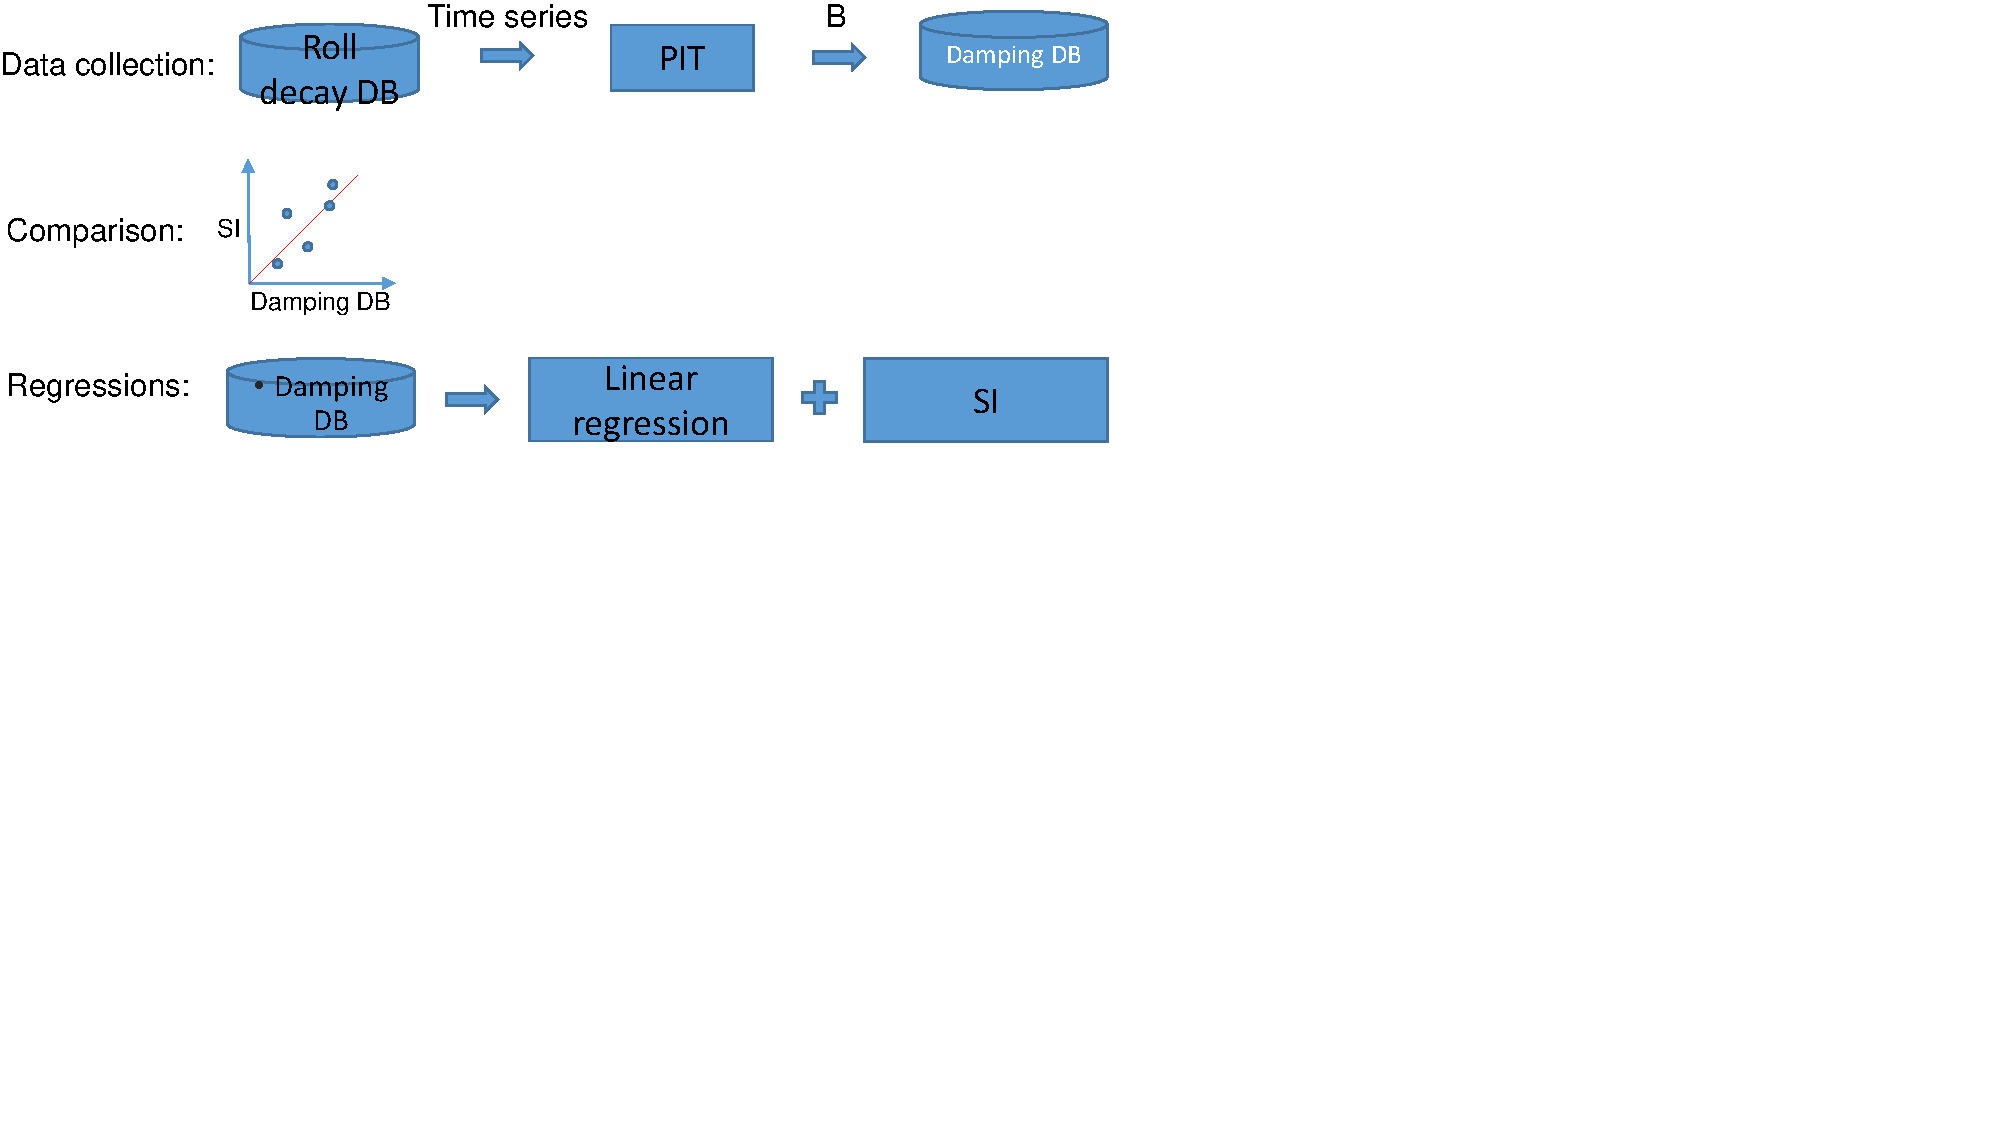
\includegraphics[width=0.5\columnwidth]{figures/workflow.pdf}
    \caption{Overview of the work conducted for this paper.}
    \label{fig:workflow}
\end{figure}